\documentclass[11pt,a4paper]{article}
\usepackage[utf8]{inputenc}\usepackage[T1]{fontenc}
\usepackage[spanish,es-noshorthands,es-noquoting]{babel}
\usepackage[margin=1.8cm]{geometry}
\usepackage{graphicx,booktabs,xcolor,tcolorbox,enumitem,textcomp,tikz,array}
\usetikzlibrary{arrows.meta,positioning}
\tcbuselibrary{skins,breakable}
\definecolor{azul}{HTML}{24618C}\definecolor{rojo}{HTML}{C0392B}\definecolor{verde}{HTML}{27632A}
\newtcolorbox{aviso}[1]{colback=rojo!6,colframe=rojo,fonttitle=\bfseries,title=#1,breakable,left=3mm,right=3mm,top=2mm,bottom=2mm}
\newtcolorbox{nota}[1]{colback=azul!6,colframe=azul,fonttitle=\bfseries,title=#1,breakable,left=3mm,right=3mm,top=2mm,bottom=2mm}
\newtcolorbox{truco}[1]{colback=verde!6,colframe=verde,fonttitle=\bfseries,title=#1,breakable,left=3mm,right=3mm,top=2mm,bottom=2mm}
\setlength{\parskip}{4pt}\pagestyle{empty}
\newcommand{\cod}[1]{\texttt{#1}}
\begin{document}
\begin{center}
{\LARGE\bfseries El modo aut\'onomo, explicado con tres diagramas}\\[1.5mm]
{\small DaVinci Paddle Boat \textperiodcentered{} Reto EIA 2027 \textperiodcentered{} Marymount}
\end{center}

\begin{nota}{De d\'onde sale y para qu\'e sirve}
Este documento explica el firmware \cod{auto\_mode\_xbox\_controller/main/sketch.cpp}. Los
tres diagramas son interactivos (con zoom y b\'usqueda) en
\cod{auto\_mode\_docs/diagramas/*.archify.html}; aqu\'i van impresos. El detalle l\'inea por
l\'inea de las variables est\'a en \cod{AUTO\_MODE\_SKETCH.md}.

\textbf{Estado:} el c\'odigo compila, pero \textbf{no se ha probado en el barco}. Todos los
n\'umeros de calibraci\'on (\cod{STEER\_KP}, 70\textdegree, tiempos) son primeras
estimaciones.
\end{nota}

%--------------------------------------------------------------------
\section*{0. Conceptos previos}

Cuatro ideas que se usan en todo el documento. Cada una termina con \emph{d\'onde aparece en
este barco}.

\subsection*{Lazo abierto}
Se da una orden y \textbf{no se comprueba} qu\'e pas\'o. El sistema conf\'ia en que la orden basta.
Ejemplo cotidiano: abrir el grifo ``un minuto'' para llenar un balde, sin mirar el balde.

\begin{center}
\begin{tikzpicture}[>=Stealth,node distance=13mm,
  b/.style={draw,rounded corners,minimum height=8mm,minimum width=22mm,fill=azul!8,font=\small}]
\node[b] (o) {Orden};
\node[b,right=of o] (a) {Actuador};
\node[b,right=of a,fill=verde!10] (p) {Barco};
\draw[->] (o)--(a); \draw[->] (a)--(p);
\end{tikzpicture}
\end{center}

\emph{En el barco:} los tiempos. \emph{``Recto durante 4 s''} y \emph{``empieza el giro''} son lazo abierto:
el barco no sabe d\'onde est\'a la boya, solo cuenta segundos. Tambi\'en lo es el \'angulo del tim\'on: el
firmware ordena un pulso de servo, pero no mide el \'angulo real del tim\'on.

\subsection*{Lazo cerrado (realimentaci\'on)}
Se \textbf{mide el resultado}, se compara con lo que se quer\'ia y se corrige. La diferencia se llama
\emph{error}. Ejemplo: un termostato, o conducir mirando la l\'inea de la carretera.

\begin{center}
\begin{tikzpicture}[>=Stealth,node distance=11mm,
  b/.style={draw,rounded corners,minimum height=8mm,minimum width=20mm,fill=azul!8,font=\small}]
\node[b,fill=white,draw=none] (r) {Objetivo};
\node[circle,draw,right=8mm of r,inner sep=1pt] (s) {$-$};
\node[b,right=of s] (c) {Controlador};
\node[b,right=of c] (a) {Actuador};
\node[b,right=of a,fill=verde!10] (p) {Barco};
\node[b,below=8mm of c,fill=rojo!8] (m) {Sensor};
\draw[->] (r)--(s); \draw[->] (s)--node[above,font=\scriptsize]{error}(c);
\draw[->] (c)--(a); \draw[->] (a)--(p);
\draw[->] (p.south) |- (m.east); \draw[->] (m.west) -| (s.south);
\end{tikzpicture}
\end{center}

\emph{En el barco:} dos lugares.
\begin{itemize}[nosep]
\item \textbf{Mantener el rumbo:} el objetivo es el rumbo de referencia, el sensor es el giroscopio y el
      controlador es \cod{steer} $=-\cod{STEER\_KP}\times$ error. Es un controlador \emph{proporcional}:
      cuanto m\'as desviado, m\'as tim\'on.
\item \textbf{El giro:} el tim\'on va fijo en $+0.6$ y el estado termina cuando el giroscopio mide 70\textdegree,
      no cuando pasa un tiempo. El tiempo (3 s) queda solo como red de seguridad.
\end{itemize}

\begin{nota}{Por qu\'e importa aqu\'i}
La direcci\'on del barco no responde de forma perfectamente predecible: se desv\'ia. Un giro por tiempo
(lazo abierto) hereda ese error; un giro por \'angulo medido (lazo cerrado) lo corrige, siempre que el
sensor funcione. Por eso el modo aut\'onomo mezcla los dos: el \emph{cu\'ando} sigue en lazo abierto, el
\emph{c\'omo} pasa a lazo cerrado.
\end{nota}

\subsection*{Giroscopio}
Mide \textbf{qu\'e tan r\'apido gira} el sensor, en grados por segundo (\textdegree/s), alrededor de un eje.
No dice hacia d\'onde apunta, solo cu\'anto est\'a girando ahora mismo.

Para obtener un \'angulo hay que \textbf{integrar}: sumar velocidad $\times$ tiempo en cada ciclo,
\[
\text{rumbo}\;\mathrel{+}=\;\text{giro}\,[\text{\textdegree/s}]\times dt\,[\text{s}].
\]
Dos problemas t\'ipicos:
\begin{itemize}[nosep]
\item \textbf{Sesgo (bias):} en reposo el giroscopio no marca exactamente 0. Por eso, al encender, se
      promedian 200 lecturas con el barco quieto y se resta ese valor (\cod{gyroZBiasRaw}).
\item \textbf{Deriva:} un error peque\~no, sumado durante mucho tiempo, crece. El rumbo integrado se
      va corriendo despacio; es aceptable en una corrida corta, no en minutos.
\end{itemize}
\emph{En el barco:} se usa solo el eje \textbf{Z} (giro horizontal, ``guiñada'' o \emph{yaw}), con rango
$\pm250$\,\textdegree/s: $131$ cuentas $=1$\,\textdegree/s. El sensor debe ir plano, con Z vertical.

\subsection*{Aceler\'ometro}
Mide la \textbf{aceleraci\'on} (m/s$^2$ o en g) en tres ejes, y siempre incluye la gravedad. Quieto sobre una
mesa marca 1\,g hacia abajo. Sirve para dos cosas:
\begin{itemize}[nosep]
\item \textbf{Inclinaci\'on:} la direcci\'on de la gravedad dice cu\'anto est\'a inclinado el barco (cabeceo y balanceo).
\item \textbf{Golpes y arranques:} detecta cambios bruscos de velocidad.
\end{itemize}
\textbf{No sirve bien para posici\'on:} habr\'ia que integrar dos veces (aceleraci\'on $\to$ velocidad $\to$
posici\'on) y el error crece muy r\'apido. Adem\'as, en un barco las olas y la vibraci\'on del motor lo llenan de
ruido. Tampoco da el rumbo horizontal: girar sobre un eje vertical no cambia la gravedad que siente.

\begin{center}\begin{tabular}{@{}>{\raggedright\arraybackslash}p{3.2cm}>{\raggedright\arraybackslash}p{4.6cm}>{\raggedright\arraybackslash}p{4.9cm}@{}}\toprule
 & \textbf{Giroscopio} & \textbf{Aceler\'ometro} \\ \midrule
Mide & velocidad de giro (\textdegree/s) & aceleraci\'on lineal + gravedad \\
Da, tras integrar & \'angulo (rumbo) & velocidad y posici\'on (con mucho error) \\
Punto d\'ebil & deriva lenta & ruido y vibraci\'on \\
Buen para & girar y mantener rumbo & inclinaci\'on, golpes \\
\textbf{En este sketch} & \textbf{s\'i, eje Z} & \textbf{no se lee} \\ \bottomrule
\end{tabular}\end{center}

El MPU-6050 trae ambos (6 ejes en total: 3 de giroscopio y 3 de aceler\'ometro), pero el firmware
aprovecha solo el giroscopio Z. Un sensor de rumbo absoluto (br\'ujula) o de posici\'on (GPS) resolver\'ia el
\emph{cu\'ando}; ninguno de los dos est\'a en el barco.

%--------------------------------------------------------------------
\section*{1. Los estados del modo aut\'onomo}

\begin{center}
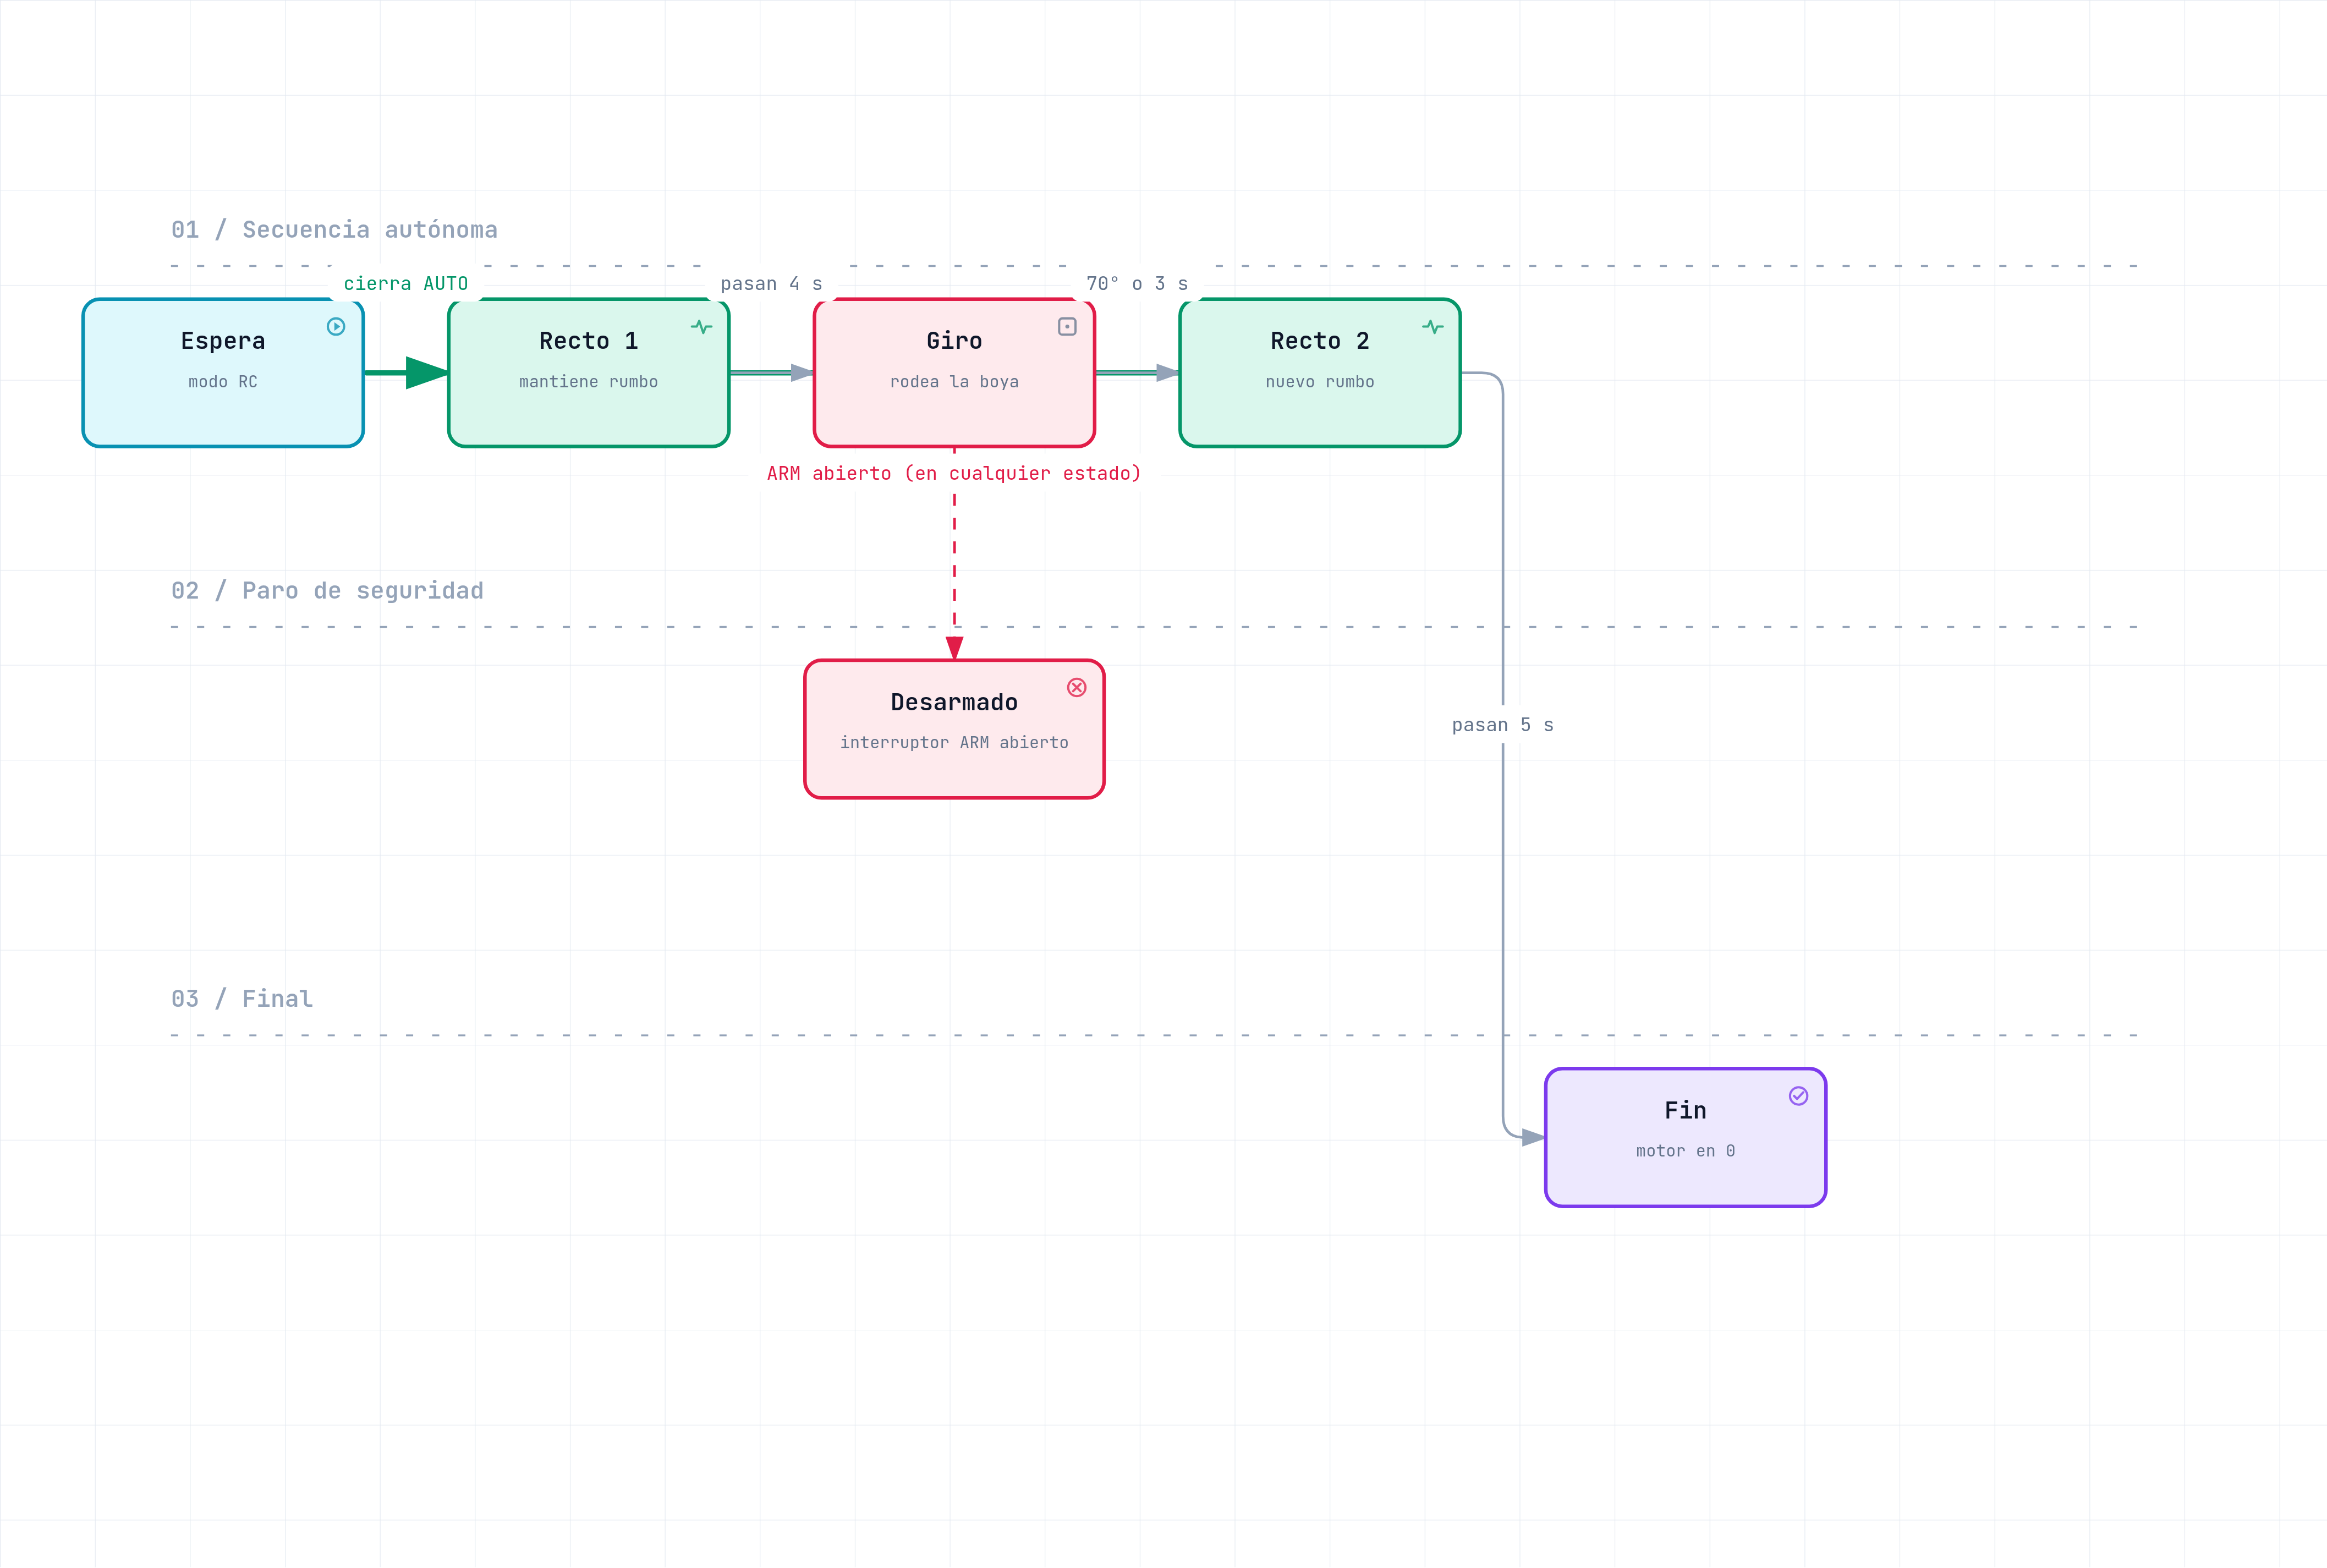
\includegraphics[width=0.8\textwidth,trim=0 0 0 300,clip]{estados-auto.png}
\end{center}

El barco recorre una secuencia fija de cuatro pasos. Al cerrar el interruptor
\textbf{AUTO} (pin 26) arranca en \emph{Recto 1}; al abrirlo vuelve a control remoto.

\begin{center}\begin{tabular}{@{}llp{7.6cm}@{}}\toprule
\textbf{Estado} & \textbf{Qu\'e hace} & \textbf{Cu\'ando termina} \\ \midrule
Recto 1 & throttle 1.0, mantiene el rumbo & pasan 4 s (\cod{STRAIGHT1\_MS\_CAP}) \\
Giro & throttle 1.0, timón fijo en $+0.6$ & el giroscopio mide 70\textdegree{} (\cod{TURN\_TARGET\_DEG}), o pasan 3 s si el sensor falla \\
Recto 2 & throttle 1.0, mantiene el nuevo rumbo & pasan 5 s (\cod{STRAIGHT2\_MS\_CAP}) \\
Fin & motor y tim\'on en 0 & no termina: hay que abrir AUTO \\ \bottomrule
\end{tabular}\end{center}

\subsection*{Qui\'en decide qu\'e}
\begin{itemize}[nosep]
\item El \textbf{giroscopio} decide \emph{c\'omo} se ejecuta cada tramo: mantener el rumbo y girar exactamente 70\textdegree.
\item Un \textbf{temporizador} decide \emph{cu\'ando} empieza el giro. El barco no tiene ning\'un sensor que le diga d\'onde est\'a la boya.
\end{itemize}

\subsection*{Mantener el rumbo}
Al empezar cada tramo recto, el rumbo actual se guarda como referencia. Cada ciclo:
\[
\text{steer} = -\,\cod{STEER\_KP}\times(\text{rumbo}-\text{referencia}),\qquad |\text{steer}|\le 0.35
\]
Con \cod{STEER\_KP} $=0.02$, estar 10\textdegree{} desviado pide $0.2$ de tim\'on. Si es muy bajo el barco
se desv\'ia; si es muy alto zigzaguea.

\begin{aviso}{El interruptor ARM manda sobre todo}
En cualquier estado, si el interruptor ARM (pin 32) est\'a abierto, el barco se desarma: motor
en 0 y tim\'on al centro. Es el paro de emergencia y tambi\'en detiene la secuencia aut\'onoma.
\end{aviso}

%--------------------------------------------------------------------
\section*{2. Un ciclo de \texttt{loop()} cada 10 ms}

\begin{center}
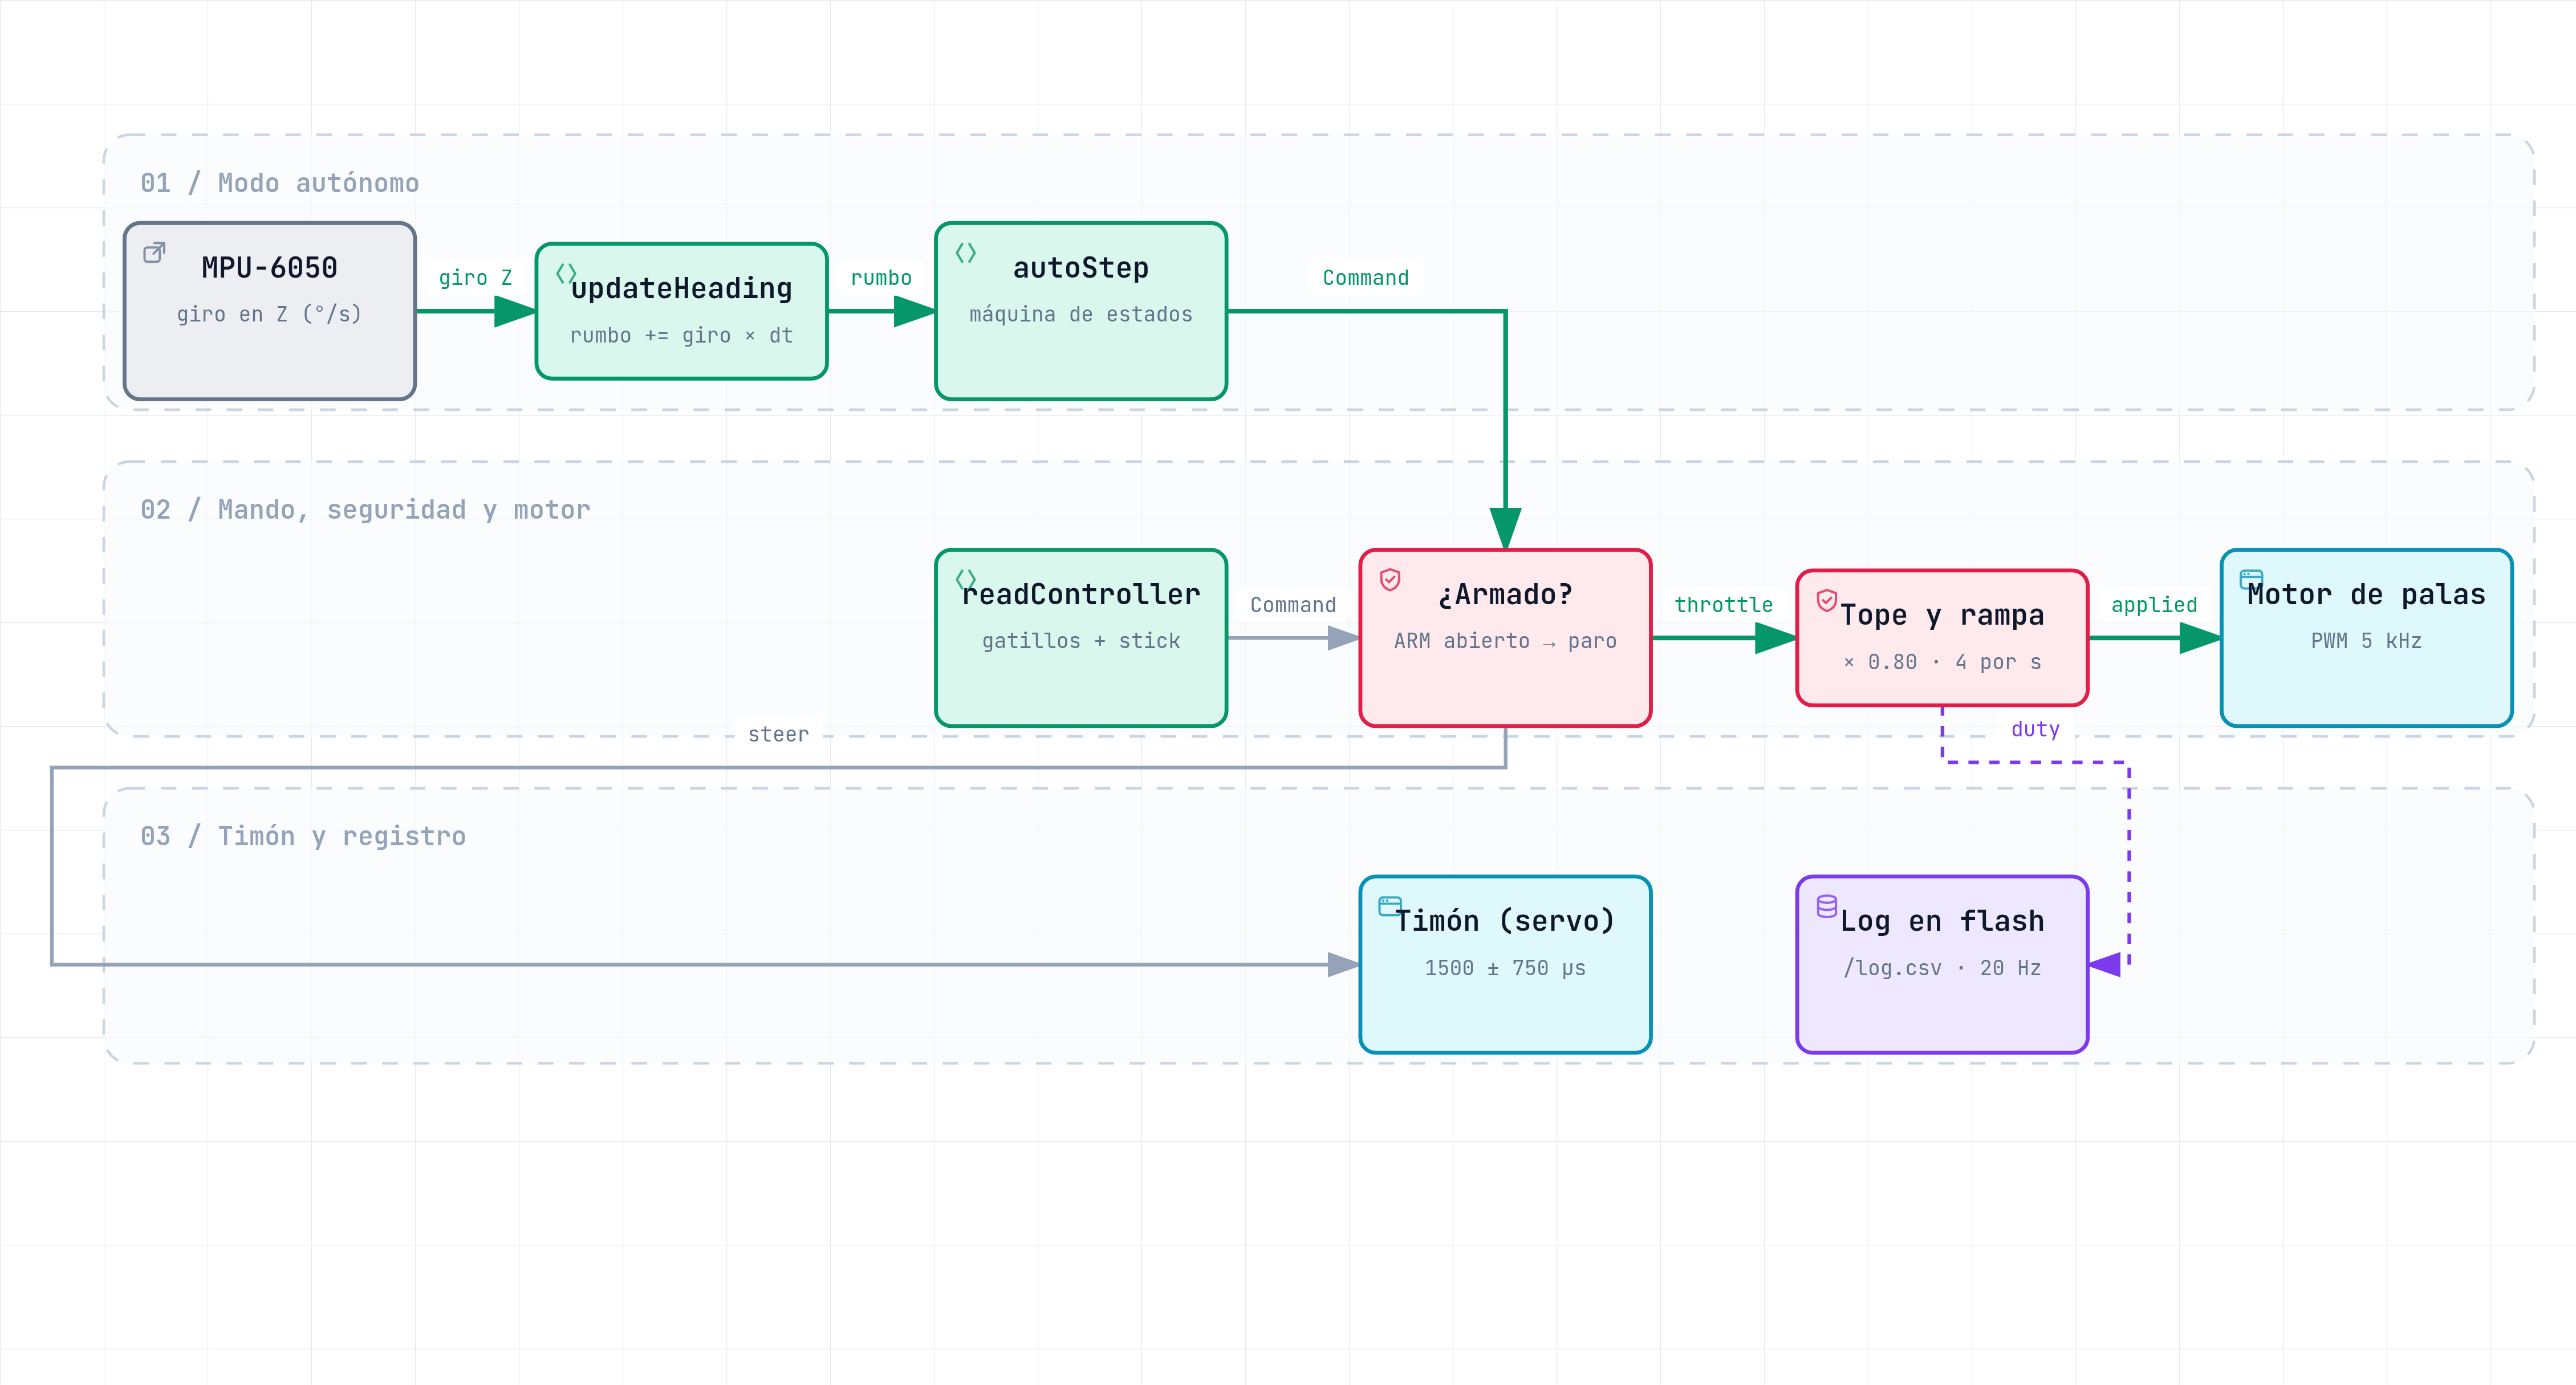
\includegraphics[width=\textwidth]{ciclo-loop.png}
\end{center}

Todo gira alrededor de una estructura, \cod{Command} (\cod{throttle}, \cod{steer}, \cod{armed}).
Dos fuentes la llenan y los actuadores solo la leen:

\begin{enumerate}[nosep]
\item \textbf{Fuente aut\'onoma:} el MPU-6050 entrega la velocidad de giro; \cod{updateHeading} la
      integra ($\text{rumbo} \mathrel{+}= \text{giro}\times dt$) y \cod{autoStep} la usa para decidir el comando.
\item \textbf{Fuente manual:} \cod{readController} lee gatillos y stick del mando Xbox.
      El interruptor AUTO elige cu\'al de las dos se usa.
\item \textbf{Seguridad:} \cod{\textquestiondown Armado?} pone \cod{armed = false} si ARM est\'a abierto.
\item \textbf{Tope y rampa:} $\text{applied}=\text{throttle}\times\cod{DUTY\_CAP}$, y el valor solo
      puede cambiar \cod{THROTTLE\_SLEW} $=4$ por segundo.
\item \textbf{Salidas:} motor de palas (PWM 5 kHz), tim\'on (pulso $1500\pm750\,\mu$s) y una fila de log.
\end{enumerate}

\begin{truco}{Un solo camino}
RC y aut\'onomo pasan por la misma seguridad y el mismo tope. Los actuadores no saben
qui\'en dio la orden, y por eso el interruptor ARM funciona igual en los dos modos.
\end{truco}

\subsection*{El tope de duty}
\cod{DUTY\_CAP} vale $0.80$: un throttle de 1.0 es 80\,\% de duty. Es un \emph{multiplicador}, no un
m\'inimo. Con menos de 80\,\% el barco no se mueve (medido), por eso todos los pasos autom\'aticos
usan throttle 1.0. El motor es de 6 V y la bater\'ia de 7.4 V, as\'i que no conviene subir ese tope.

\subsection*{C\'omo sabe cu\'anto tim\'on us\'o}
No lo mide. El firmware conoce el n\'umero porque \'el mismo lo orden\'o (\cod{cmd.steer}) y lo
guarda en el log. El giroscopio mide el \emph{resultado}: cu\'anto gir\'o el barco. Con las dos columnas
juntas se ve orden y respuesta. No hay realimentaci\'on del \'angulo real del servo.

%--------------------------------------------------------------------
\section*{3. Del agua al an\'alisis: el log sin cable}

\begin{center}
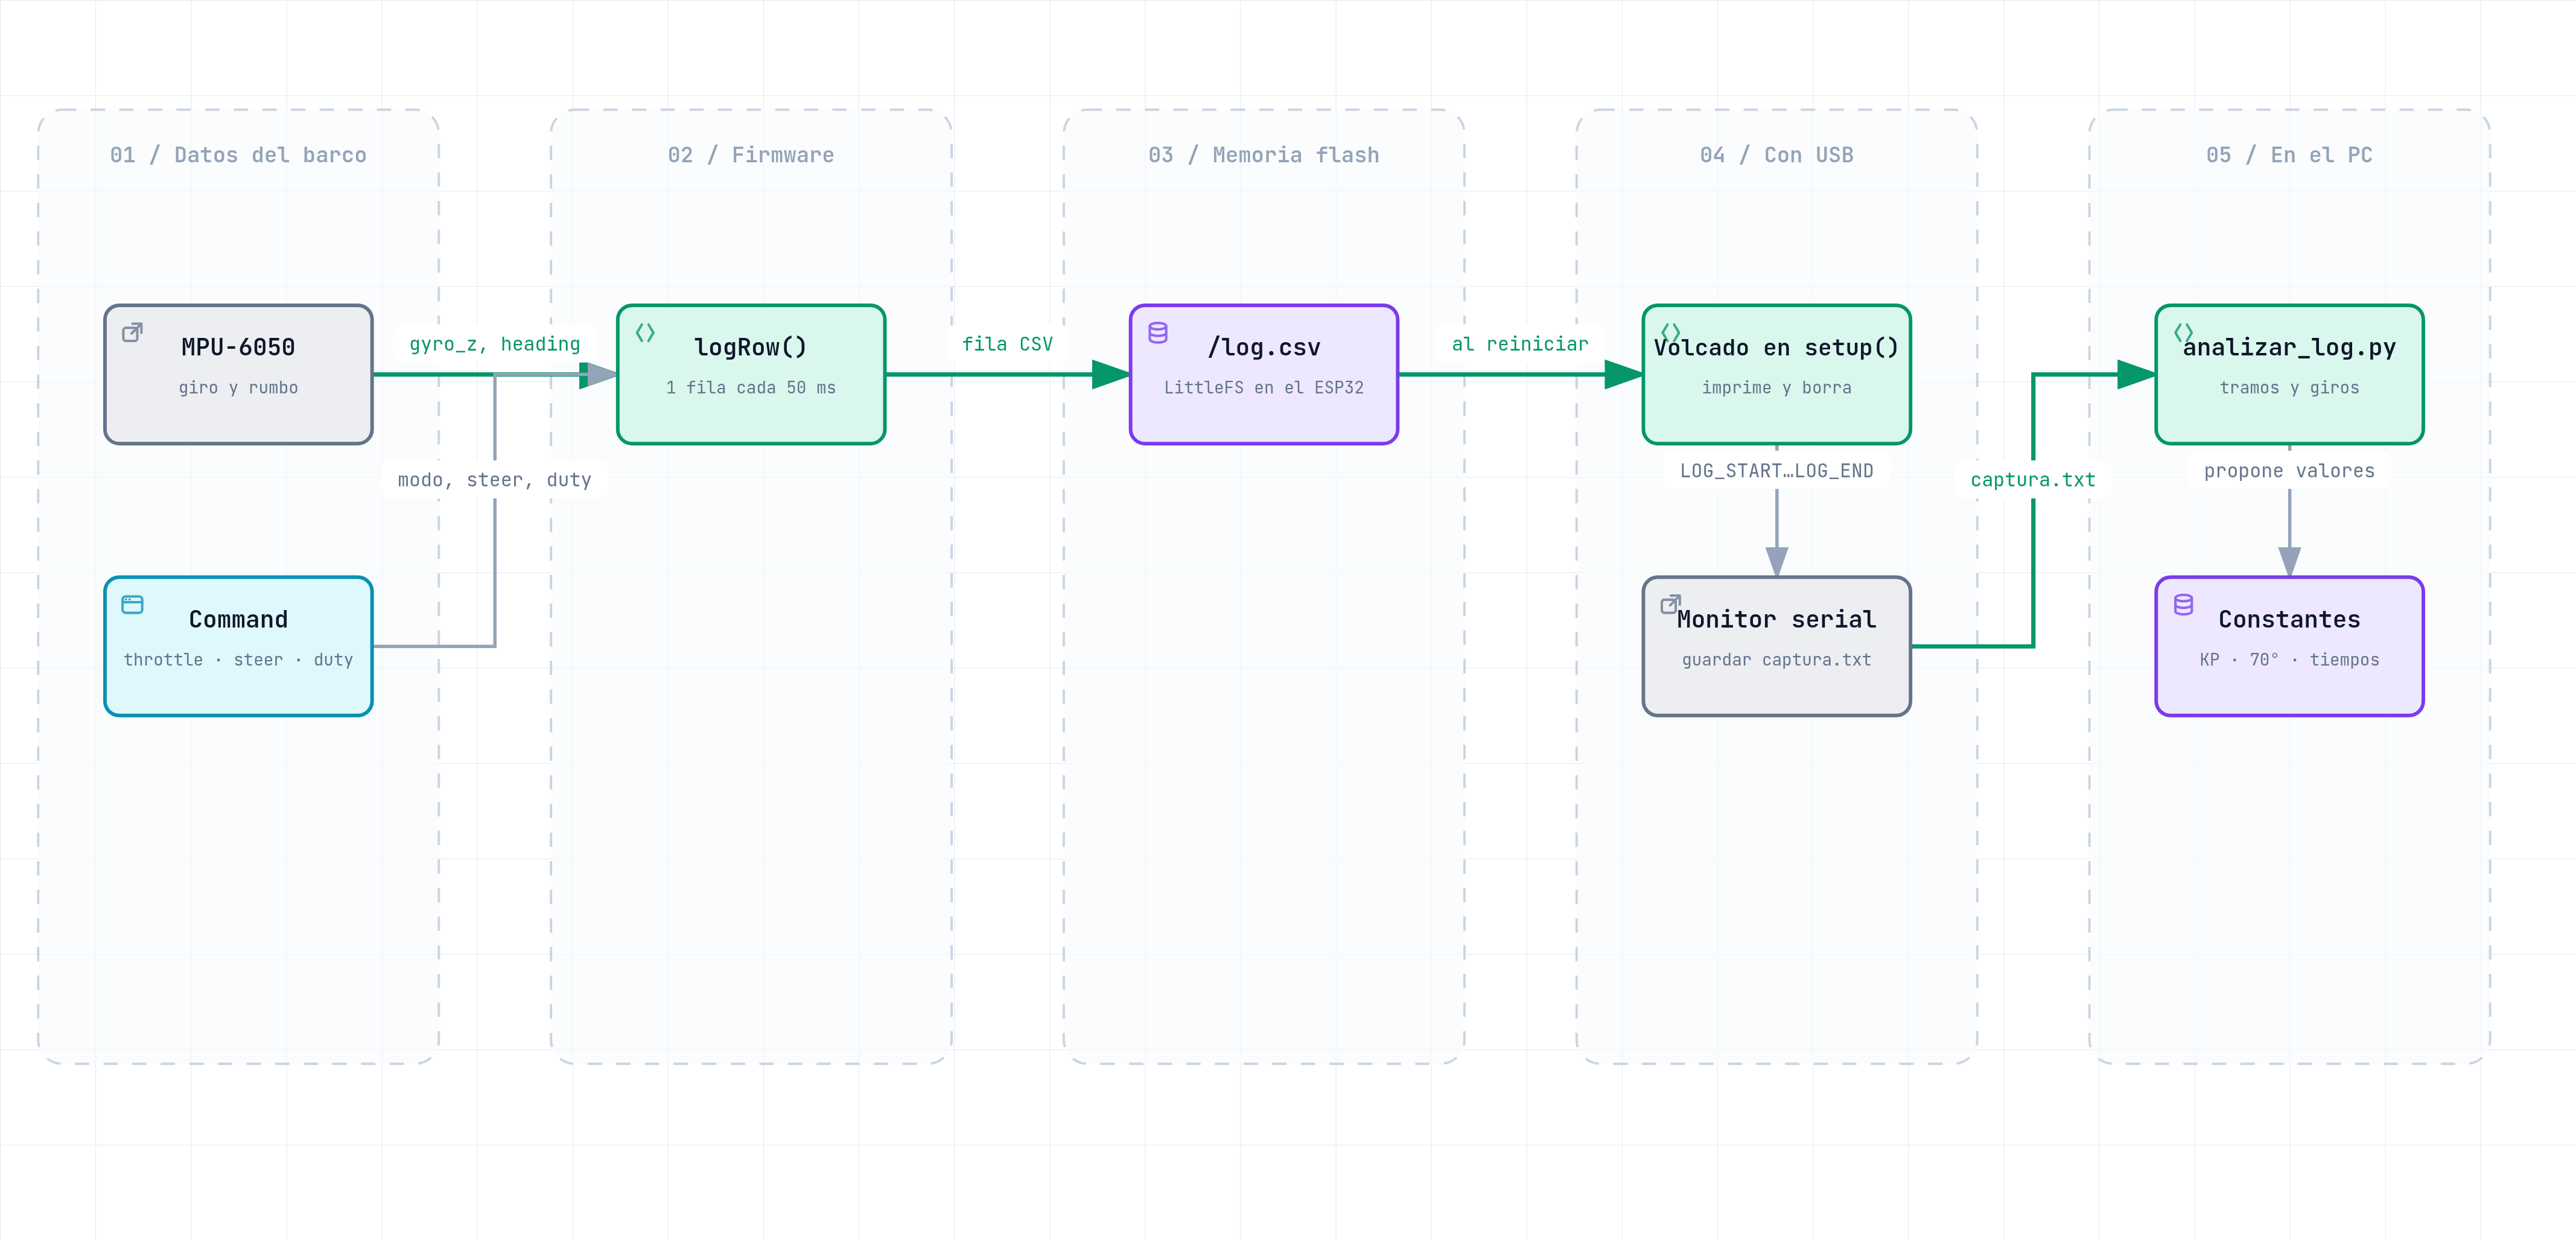
\includegraphics[width=\textwidth]{log-datos.png}
\end{center}

El barco no puede llevar un cable en el agua, as\'i que registra la prueba en su memoria flash
y se lee despu\'es.

\begin{enumerate}[nosep]
\item \textbf{Durante la prueba:} cada 50 ms (20 Hz) \cod{logRow()} escribe una fila en \cod{/log.csv}
      (LittleFS) y guarda a flash una vez por segundo.
\item \textbf{Despu\'es:} con el barco fuera del agua, se conecta el USB y se \textbf{abre el monitor serial}.
\item \textbf{Se reinicia la placa.} \cod{setup()} imprime el archivo entre \cod{===LOG\_START===} y
      \cod{===LOG\_END===} (por \cod{Console}) y \textbf{lo borra}.
\item Se guarda la salida como \cod{captura.txt} y se corre
      \cod{python3 analizar\_log.py captura.txt}, que propone valores para el sketch.
\end{enumerate}

\begin{center}\begin{tabular}{@{}ll@{}}\toprule
\textbf{Columna} & \textbf{Significado} \\ \midrule
\cod{t\_ms} & tiempo desde el arranque \\
\cod{modo} & 1 = aut\'onomo, 0 = radiocontrol \\
\cod{throttle}, \cod{steer} & la orden, antes del tope \\
\cod{gyro\_z\_dps} & velocidad de giro medida (\textdegree/s) \\
\cod{heading\_deg} & rumbo integrado, relativo al inicio del modo aut\'onomo \\
\cod{duty} & el ciclo de trabajo real aplicado (ya con tope y rampa) \\ \bottomrule
\end{tabular}\end{center}

\begin{aviso}{Cuidado: el volcado borra el archivo}
Si se reinicia la placa \emph{sin} el monitor serial abierto, esa corrida se pierde. Y si se corta la
energ\'ia durante la prueba, se pierde como m\'aximo el \'ultimo segundo. Guarda \cod{captura.txt}
antes de volver a probar.
\end{aviso}

%--------------------------------------------------------------------
\section*{Antes de la primera prueba}
\begin{itemize}[nosep]
\item Confirmar que el sensor responde (\cod{gyroOK = 1} al arrancar) y montarlo plano, con el eje Z vertical.
\item Girar el barco a mano a la derecha y comprobar que \cod{heading\_deg} \textbf{sube}; y que un
      \cod{steer} positivo gira hacia el mismo lado. Si no coinciden, la correcci\'on empuja al rev\'es.
\item Mantener el barco \textbf{quieto} al encender: ah\'i se calibra el sesgo del giroscopio.
\item Si el interruptor AUTO ya est\'a cerrado al encender, el modo aut\'onomo arranca de inmediato.
\item Calibrar los n\'umeros con el log; el giroscopio deriva lentamente, lo cual es aceptable en una corrida corta.
\end{itemize}
\end{document}
